%%% Local Variables:
%%% mode: latex
%%% TeX-master: t
%%% End:
\documentclass{beamer}
\usepackage[utf8]{inputenc}
\usepackage[german]{babel}
\usepackage{graphics}
\usepackage{listings}
\usepackage{caption}

\captionsetup{font=scriptsize,labelfont=scriptsize}

\usetheme{default}
\usecolortheme{rose}

\DeclareGraphicsRule{.pdftex}{pdf}{.pdftex}{}

% \lstdefinelanguage{cfengine}
%   {morekeywords={import,classes,control,admit,copy,editfiles,processes,shellcommands},
%    sensitive=false,
%    morecommment[l]{//},
%   }

\newcommand\Fontvi{\fontsize{6}{7.2}\selectfont}

\lstset{
basicstyle=\tiny,
stringstyle=\tiny,
numbers=left,
numberstyle=\tiny,
stepnumber=2,
frame=single,
%language=cfengine,
captionpos=b
}

\title{System Automation mit Puppet und Foreman\\}
\author{Toni Schmidbauer}

\begin{document}

\begin{frame}
\center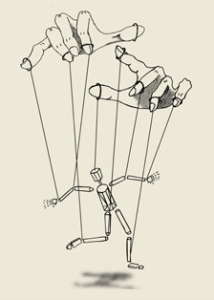
\includegraphics[height=2.5cm,width=2cm]{../pics/puppet.png}
\titlepage

\end{frame}

\begin{frame}
  \frametitle{whoami}
  \begin{itemize}
  \item SysAdmin@s-itsolutions
  \item toni@stderr.at
  \item http://github.com/tosmi
  \item stderr@jabber.org
  \end{itemize}
\end{frame}
\begin{frame}

  \frametitle{Agenda}

  \begin{itemize}
  \item Kurze Umfrage
  \item Was ist Puppet?
  \item Was ist Foreman?
  \item Puppet@s-iTSolutions
  \item Was haben wir geplant
  \end{itemize}

\end{frame}

\begin{frame}
\center{\huge{Umfrage}}
\end{frame}

\begin{frame}[fragile]
  \frametitle{Was ist Puppet?}

  \begin{lstlisting}
    class linuxwochen2014 {

      user { 'linuxwochen':
        ensure => present,
        uid => 4711,
        gid => 4711,
      }

      package { 'emacs':
        ensure => installed
      } ->
      package { 'vi':
        ensure => absent,
      }
    }
  \end{lstlisting}
\end{frame}


\begin{frame}[fragile]
  \frametitle{Zuordnung von Klassen}

  \begin{lstlisting}
    node linuxwochen {
      include mypuppetconfig
    }
  \end{lstlisting}

  \begin{itemize}
  \item oder über einen External Node Classifier (Foreman)
  \end{itemize}
\end{frame}

\begin{frame}
  \frametitle{Was ist Foreman?}
  \begin{figure}[ht]
    \centering
    \framebox{
      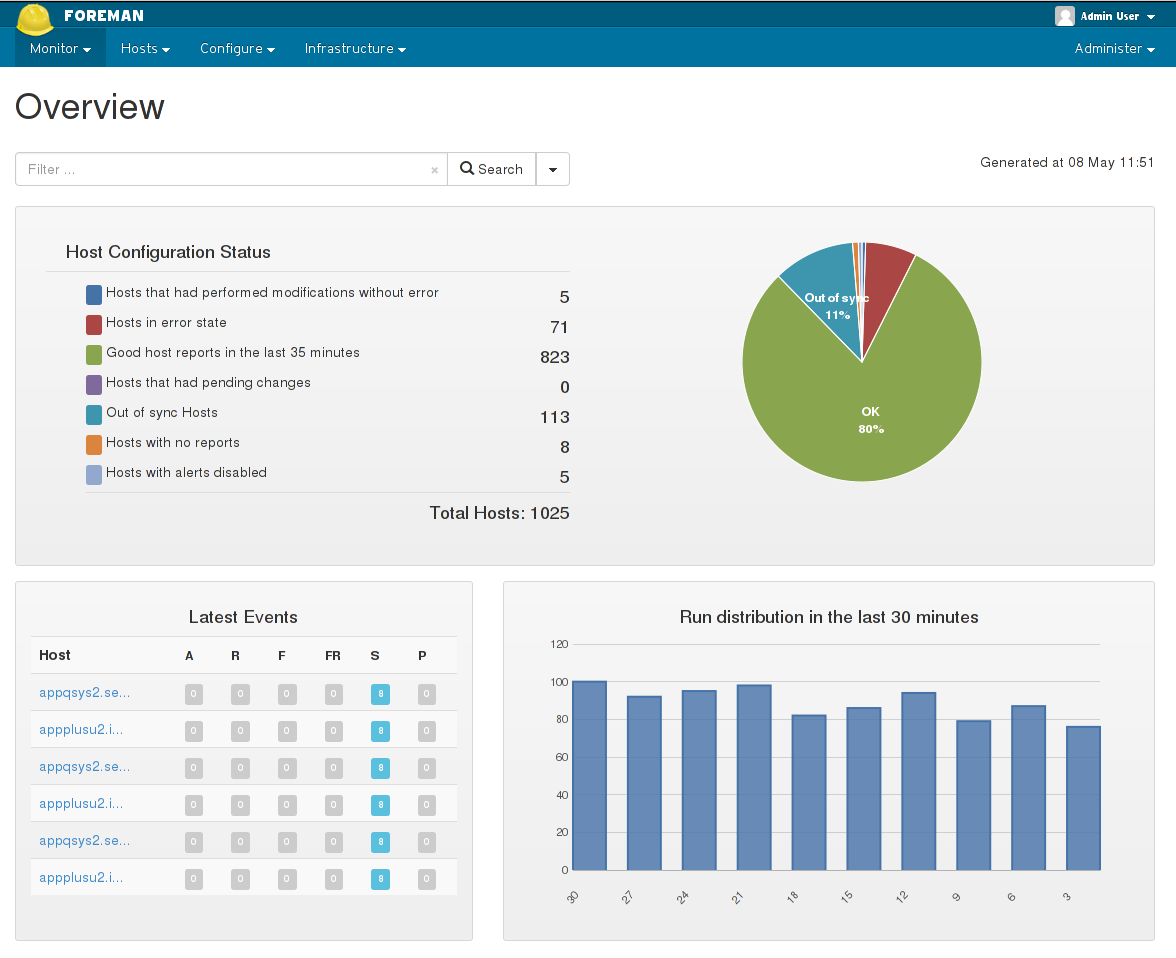
\includegraphics[height=7.5cm,width=10.3cm]{../pics/foreman_dashboard.png}
    }
    \label{fig:stack}
  \end{figure}
\end{frame}

\begin{frame}
  \frametitle{Puppet run}
  \begin{figure}[ht]
    \centering
      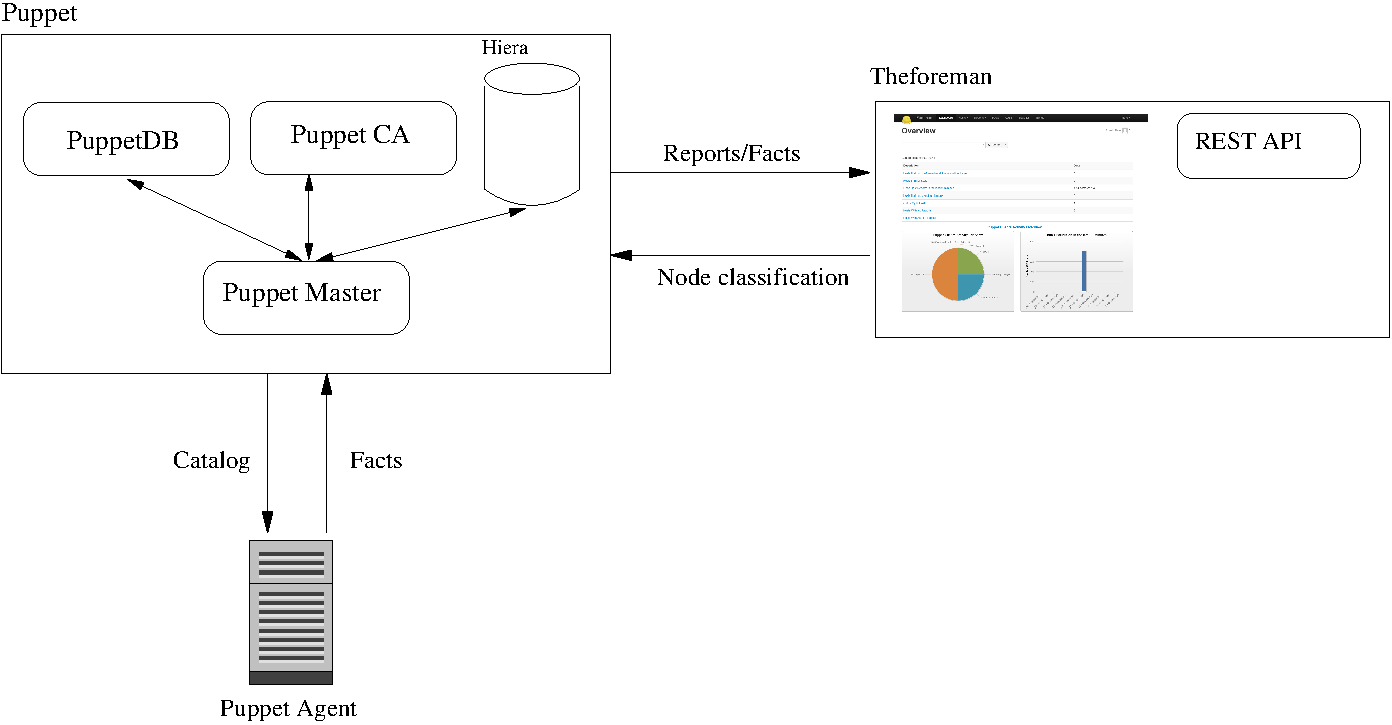
\includegraphics[height=6.5cm,width=11cm]{../pics/puppet_overview}
    \label{fig:stack}
  \end{figure}
\end{frame}

\begin{frame}
  \center{\huge{Und jetzt?}}
\end{frame}

\begin{frame}
  \begin{figure}[ht]
    \centering
      
\includegraphics[height=7.5cm,width=10cm]{../pics/chucky.png}
    \label{fig:stack}
  \end{figure}
\end{frame}


\begin{frame}
  \begin{itemize}
  \item Wie verwaltet wir unseren Puppet Code?
  \item Wie soll unsere Puppet Umgebung aussehen?
  \item Wie erfolgt das Deployment des Codes?
  \item Wie organisieren wir Module?
  \item Wie soll eine Entwicklungsumgebung aussehen?
  \item Wie testen wir den Puppet Code?
  \item Wie verwalten wir Module von PuppetForge?
  \end{itemize}
\end{frame}

\begin{frame}
  \center{\huge{Wie verwaltet wir unseren Puppet Code?}}
  \center{\huge{Wie organisieren wir Module?}}
\end{frame}

\begin{frame}
  \frametitle{GIT}

  \begin{itemize}
  \item Ein zentrales GIT Repository
  \item Berechtigungssystem für GIT mit gitolite
  \item 3 Hauptbranches
    \begin{itemize}
    \item Master: Staging via GIT pull auf 4 Dev Server
    \item Testing: ca. 25 ``Produktions'' Server (git pull)
    \item Production: der Rest, Staging via tags
    \end{itemize}
  \item Feature Branches für neue Module
  \end{itemize}
\end{frame}

\begin{frame}
  \center{\huge{Demo}}
\end{frame}

\begin{frame}
  \center{\huge{Wie soll unsere Puppet Umgebung aussehen?}}
  \center{\huge{Wie erfolgt das Deployment des Codes?}}
\end{frame}

\begin{frame}
  \frametitle{Puppet Umgebung}
  \begin{figure}[ht]
    \centering
      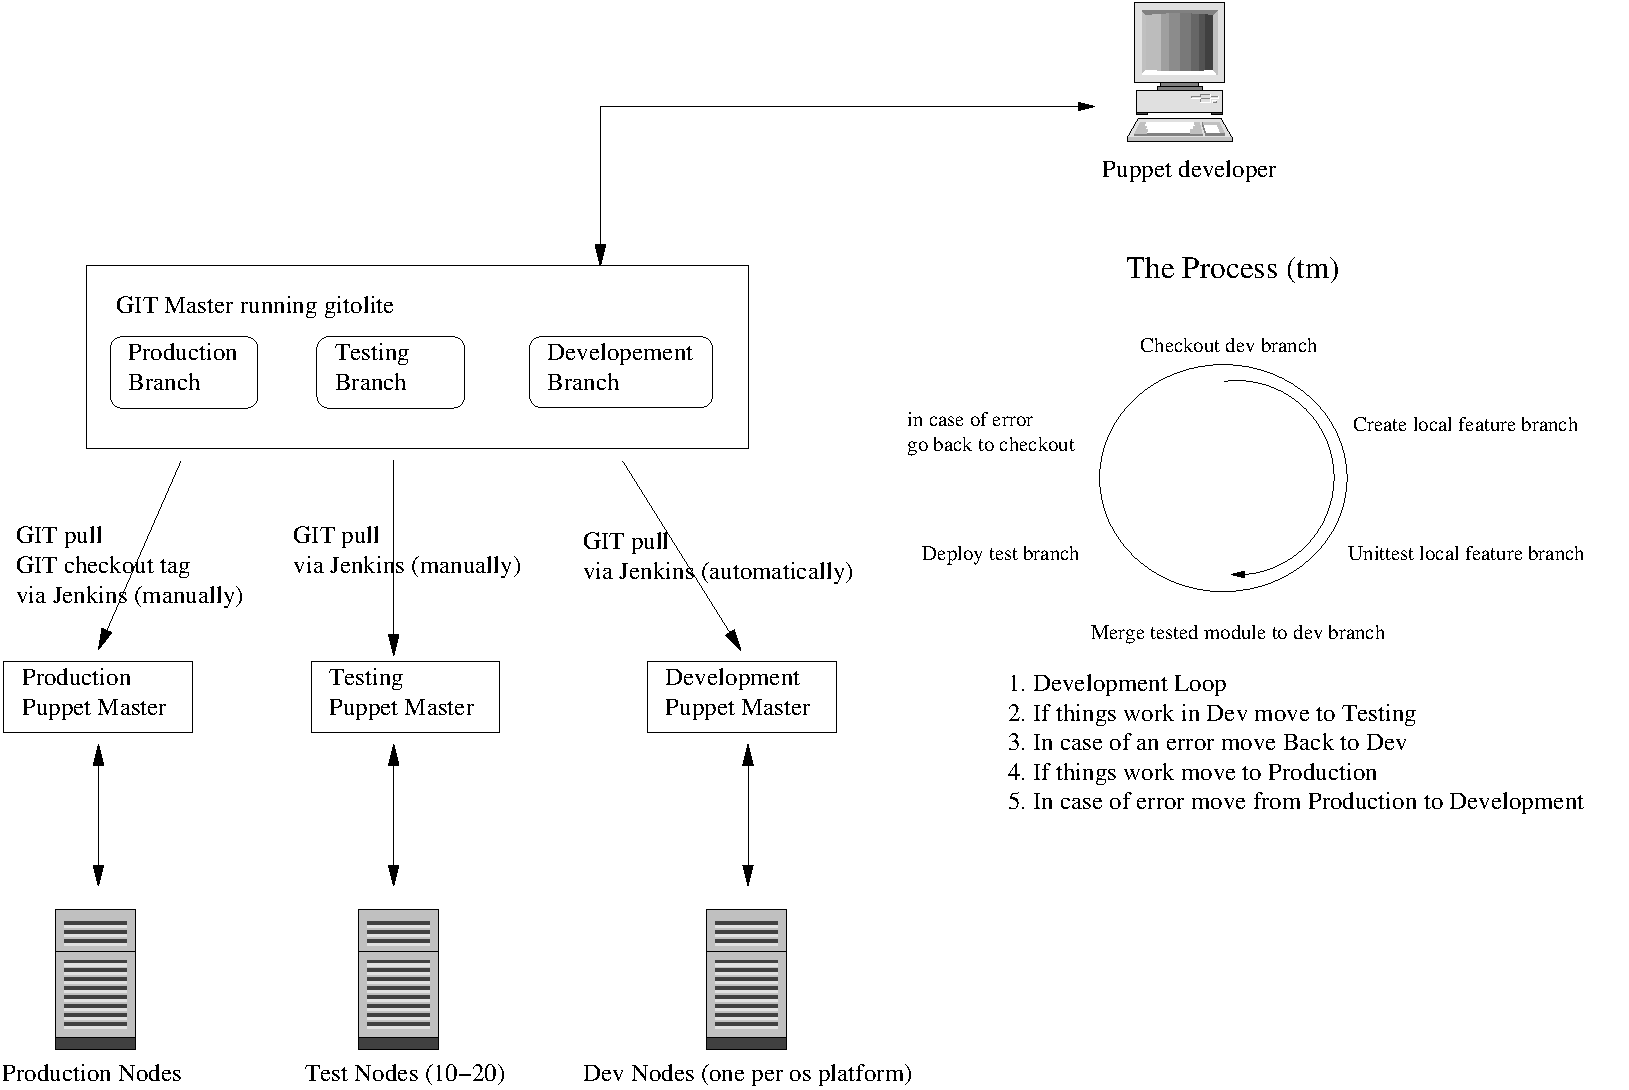
\includegraphics[height=7.2cm,width=11.5cm]{../pics/puppet_deployment}
  \end{figure}
\end{frame}

\begin{frame}
  \frametitle{Puppet Umgebung II}

  \begin{itemize}
  \item Am Development Master verwenden wir dynamische Puppet Environments \\
    \tiny{\url{http://puppetlabs.com/blog/git-workflow-and-puppet-environments}}
    \normalsize
  \item Jeder Feature Branch wird ein eigenes Puppet Environment
  \item Das Staging in die Produktion erfolgt über GIT tags
  \end{itemize}
\end{frame}

\begin{frame}
  \center{\huge{Wie soll eine Entwicklungsumgebung aussehen?}}
\end{frame}

\begin{frame}
  \begin{figure}[ht]
    \centering
      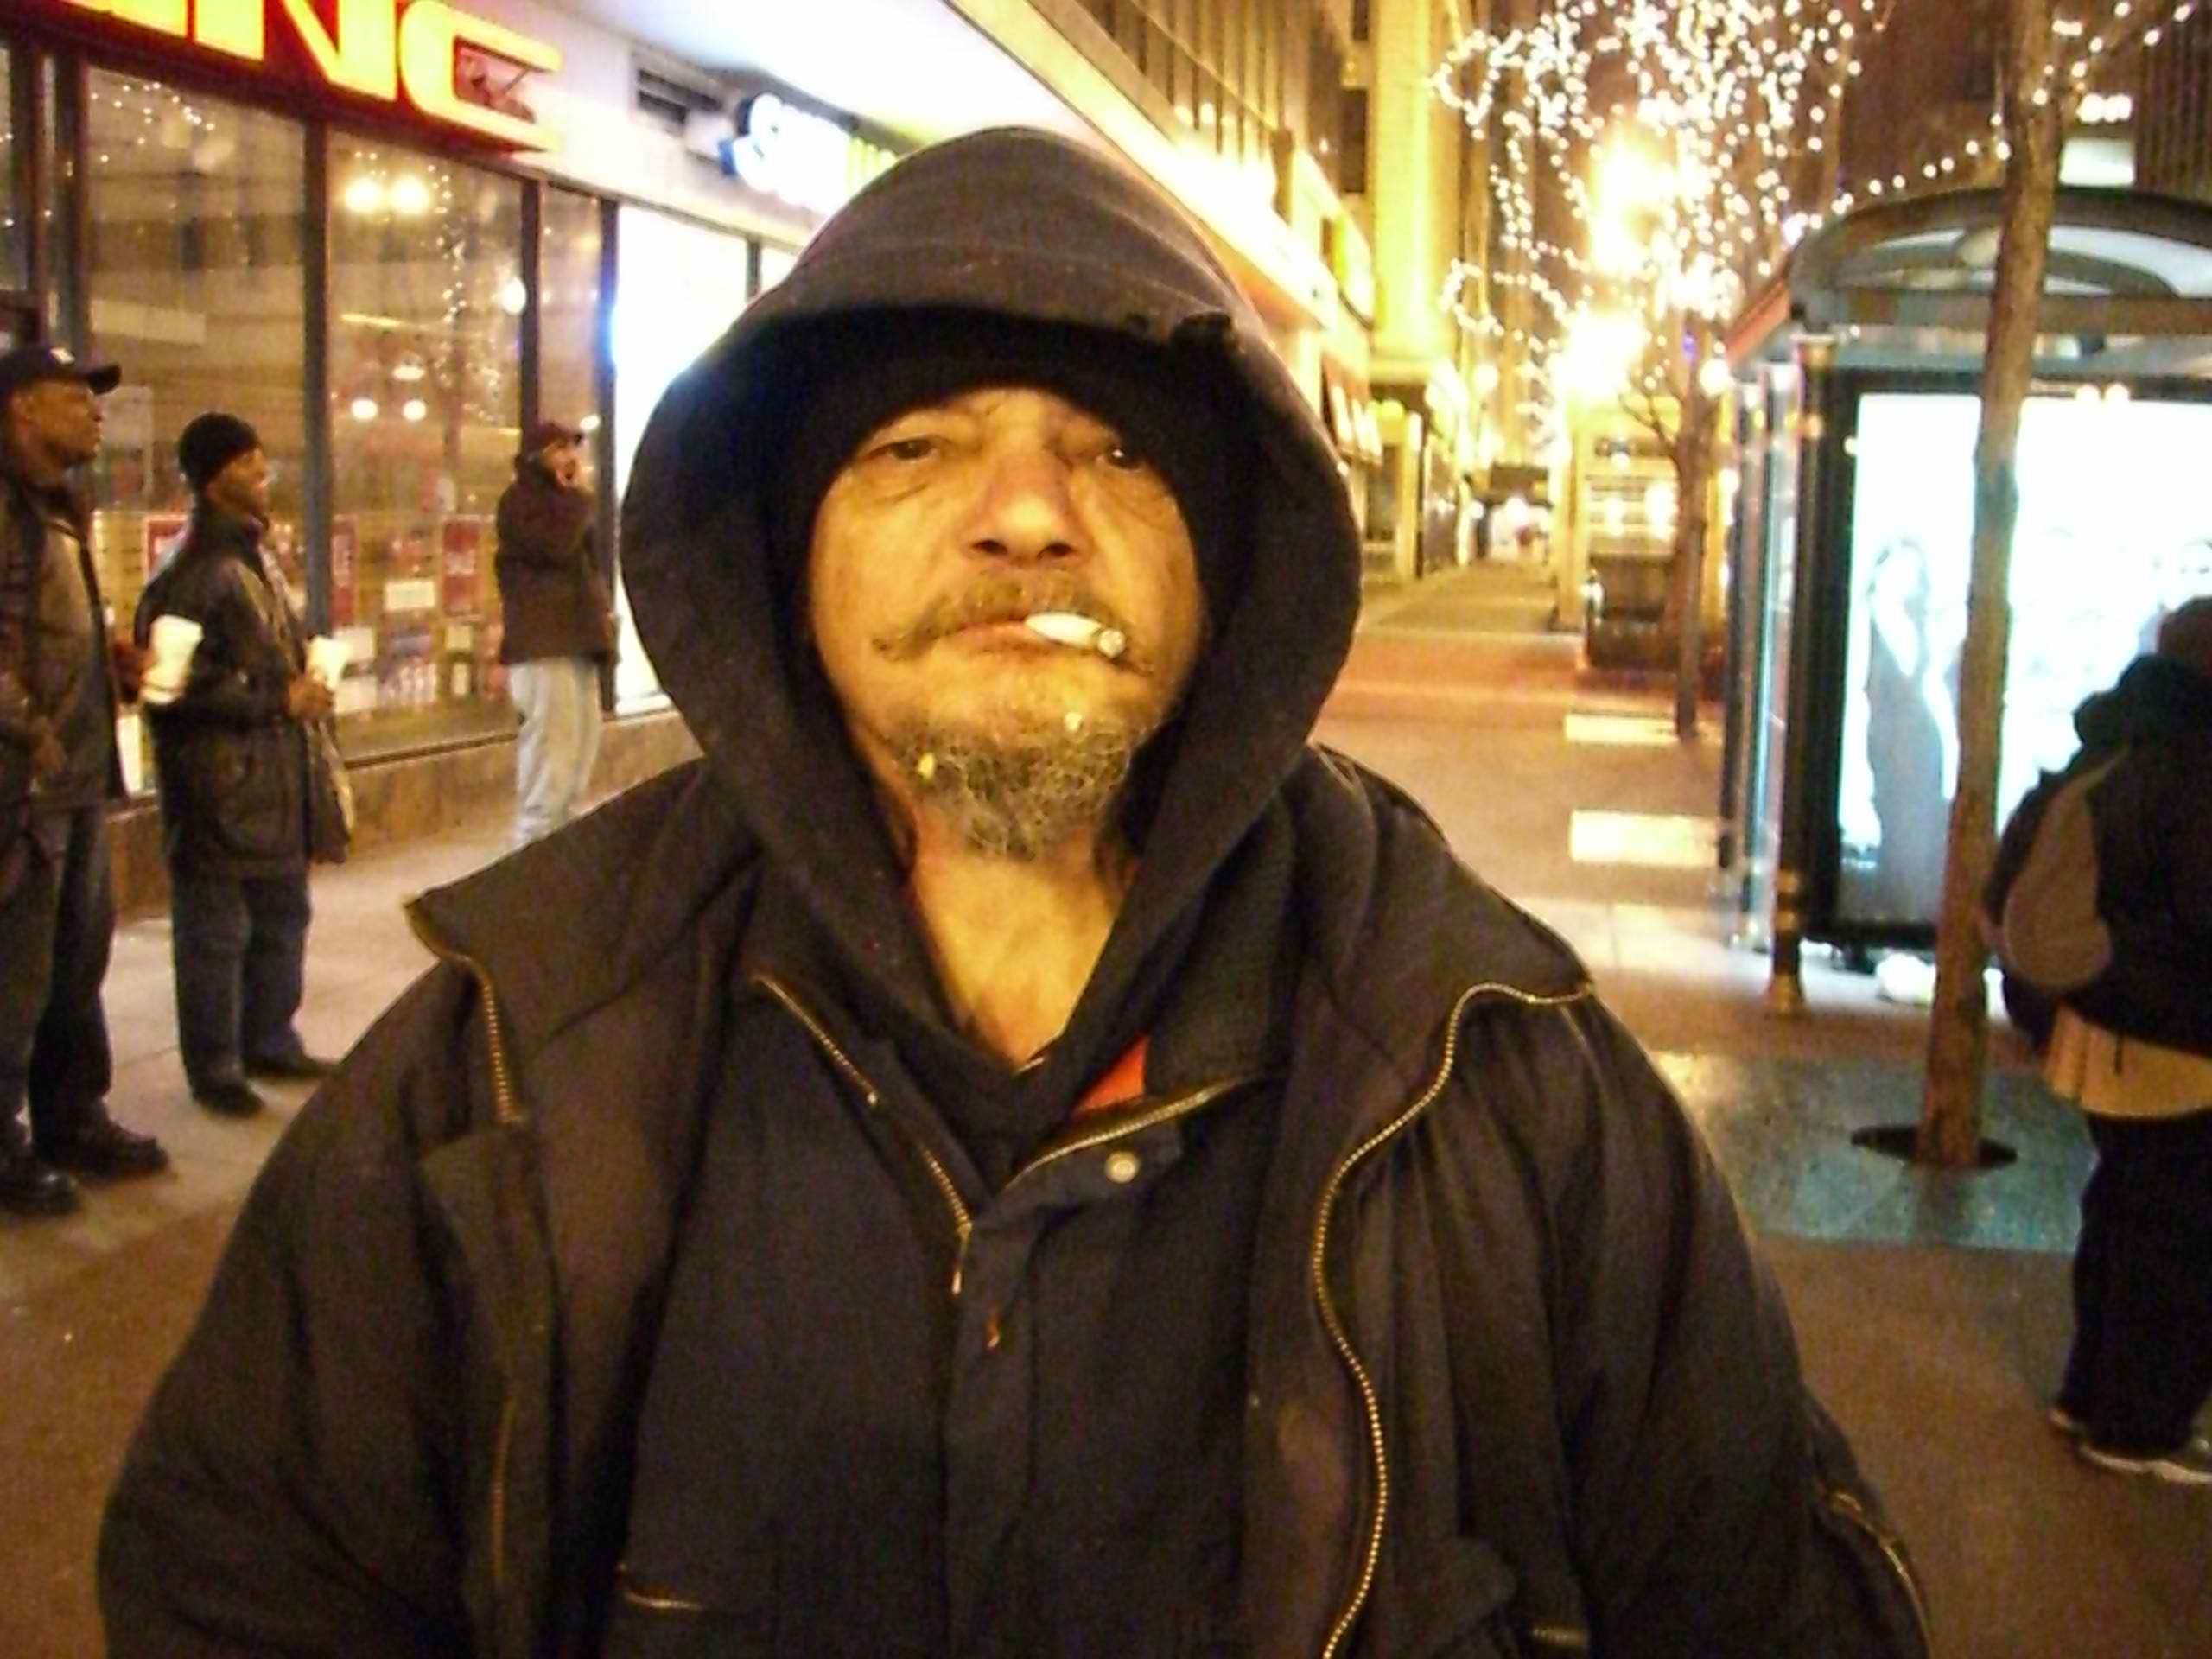
\includegraphics[height=7.5cm,width=10cm]{../pics/vagrant.png}
    \label{fig:stack}
  \end{figure}
\end{frame}

\begin{frame}
  \frametitle{Vagrant}

  \begin{itemize}
  \item \url{http://vagrantup.com}
  \item Ermöglicht virtuelle Entwicklungsumgebungen
  \item Vagrant Box ist ein vorkonfiguriertes Image
  \item Default VirtualBox andere Provider via Plugins (VMWare, KVM)
  \end{itemize}
\end{frame}

\begin{frame}
  \center{\huge{Demo}}
\end{frame}

\begin{frame}
  \center{\huge{Wie testen wir den Puppet Code?}}
\end{frame}

\begin{frame}
  \frametitle{rspec-puppet}

  \begin{itemize}
  \item Ruby RSpec Tests für Puppet
  \item Ist in unserer Vagrant Umgebung vorinstalliert
  \item Jedes Module muss RSpec Tests mitbringen
  \item Commit in Master Branch löst einen Jenkins Build aus
  \item Commit in Testing Branch löst einen Jenkins Build aus
  \item Commit in Production Branch löst einen Jenkins Build aus
  \end{itemize}
\end{frame}

\begin{frame}
  \center{\huge{Wie verwalten wir Module von PuppetForge?}}
\end{frame}

\begin{frame}
  \frametitle{Puppetforge Module}

  \begin{itemize}
  \item Eigenes GIT Repository (puppetforge.git)
  \item Download der Module in der Enwicklungsumgebung
  \item Staging wie unser Haupt Puppet Repository
  \end{itemize}
\end{frame}

\begin{frame}
  \begin{itemize}
  \item Wie verwaltet wir unseren Puppet Code? \emph{\color{green}DONE}
  \item Wie soll unsere Puppet Umgebung aussehen?  \emph{\color{green}DONE}
  \item Wie erfolgt das Deployment des Codes? \emph{\color{green}DONE}
  \item Wie organisieren wir Module? \emph{\color{green}DONE}
  \item Wie soll eine Entwicklungsumgebung aussehen? \emph{\color{green}DONE}
  \item Wie testen wir den Puppet Code? \emph{\color{green}DONE}
  \item Wie verwalten wir Module von PuppetForge? \emph{\color{green}DONE}
  \end{itemize}
\end{frame}

\begin{frame}
  \begin{figure}[ht]
    \centering
      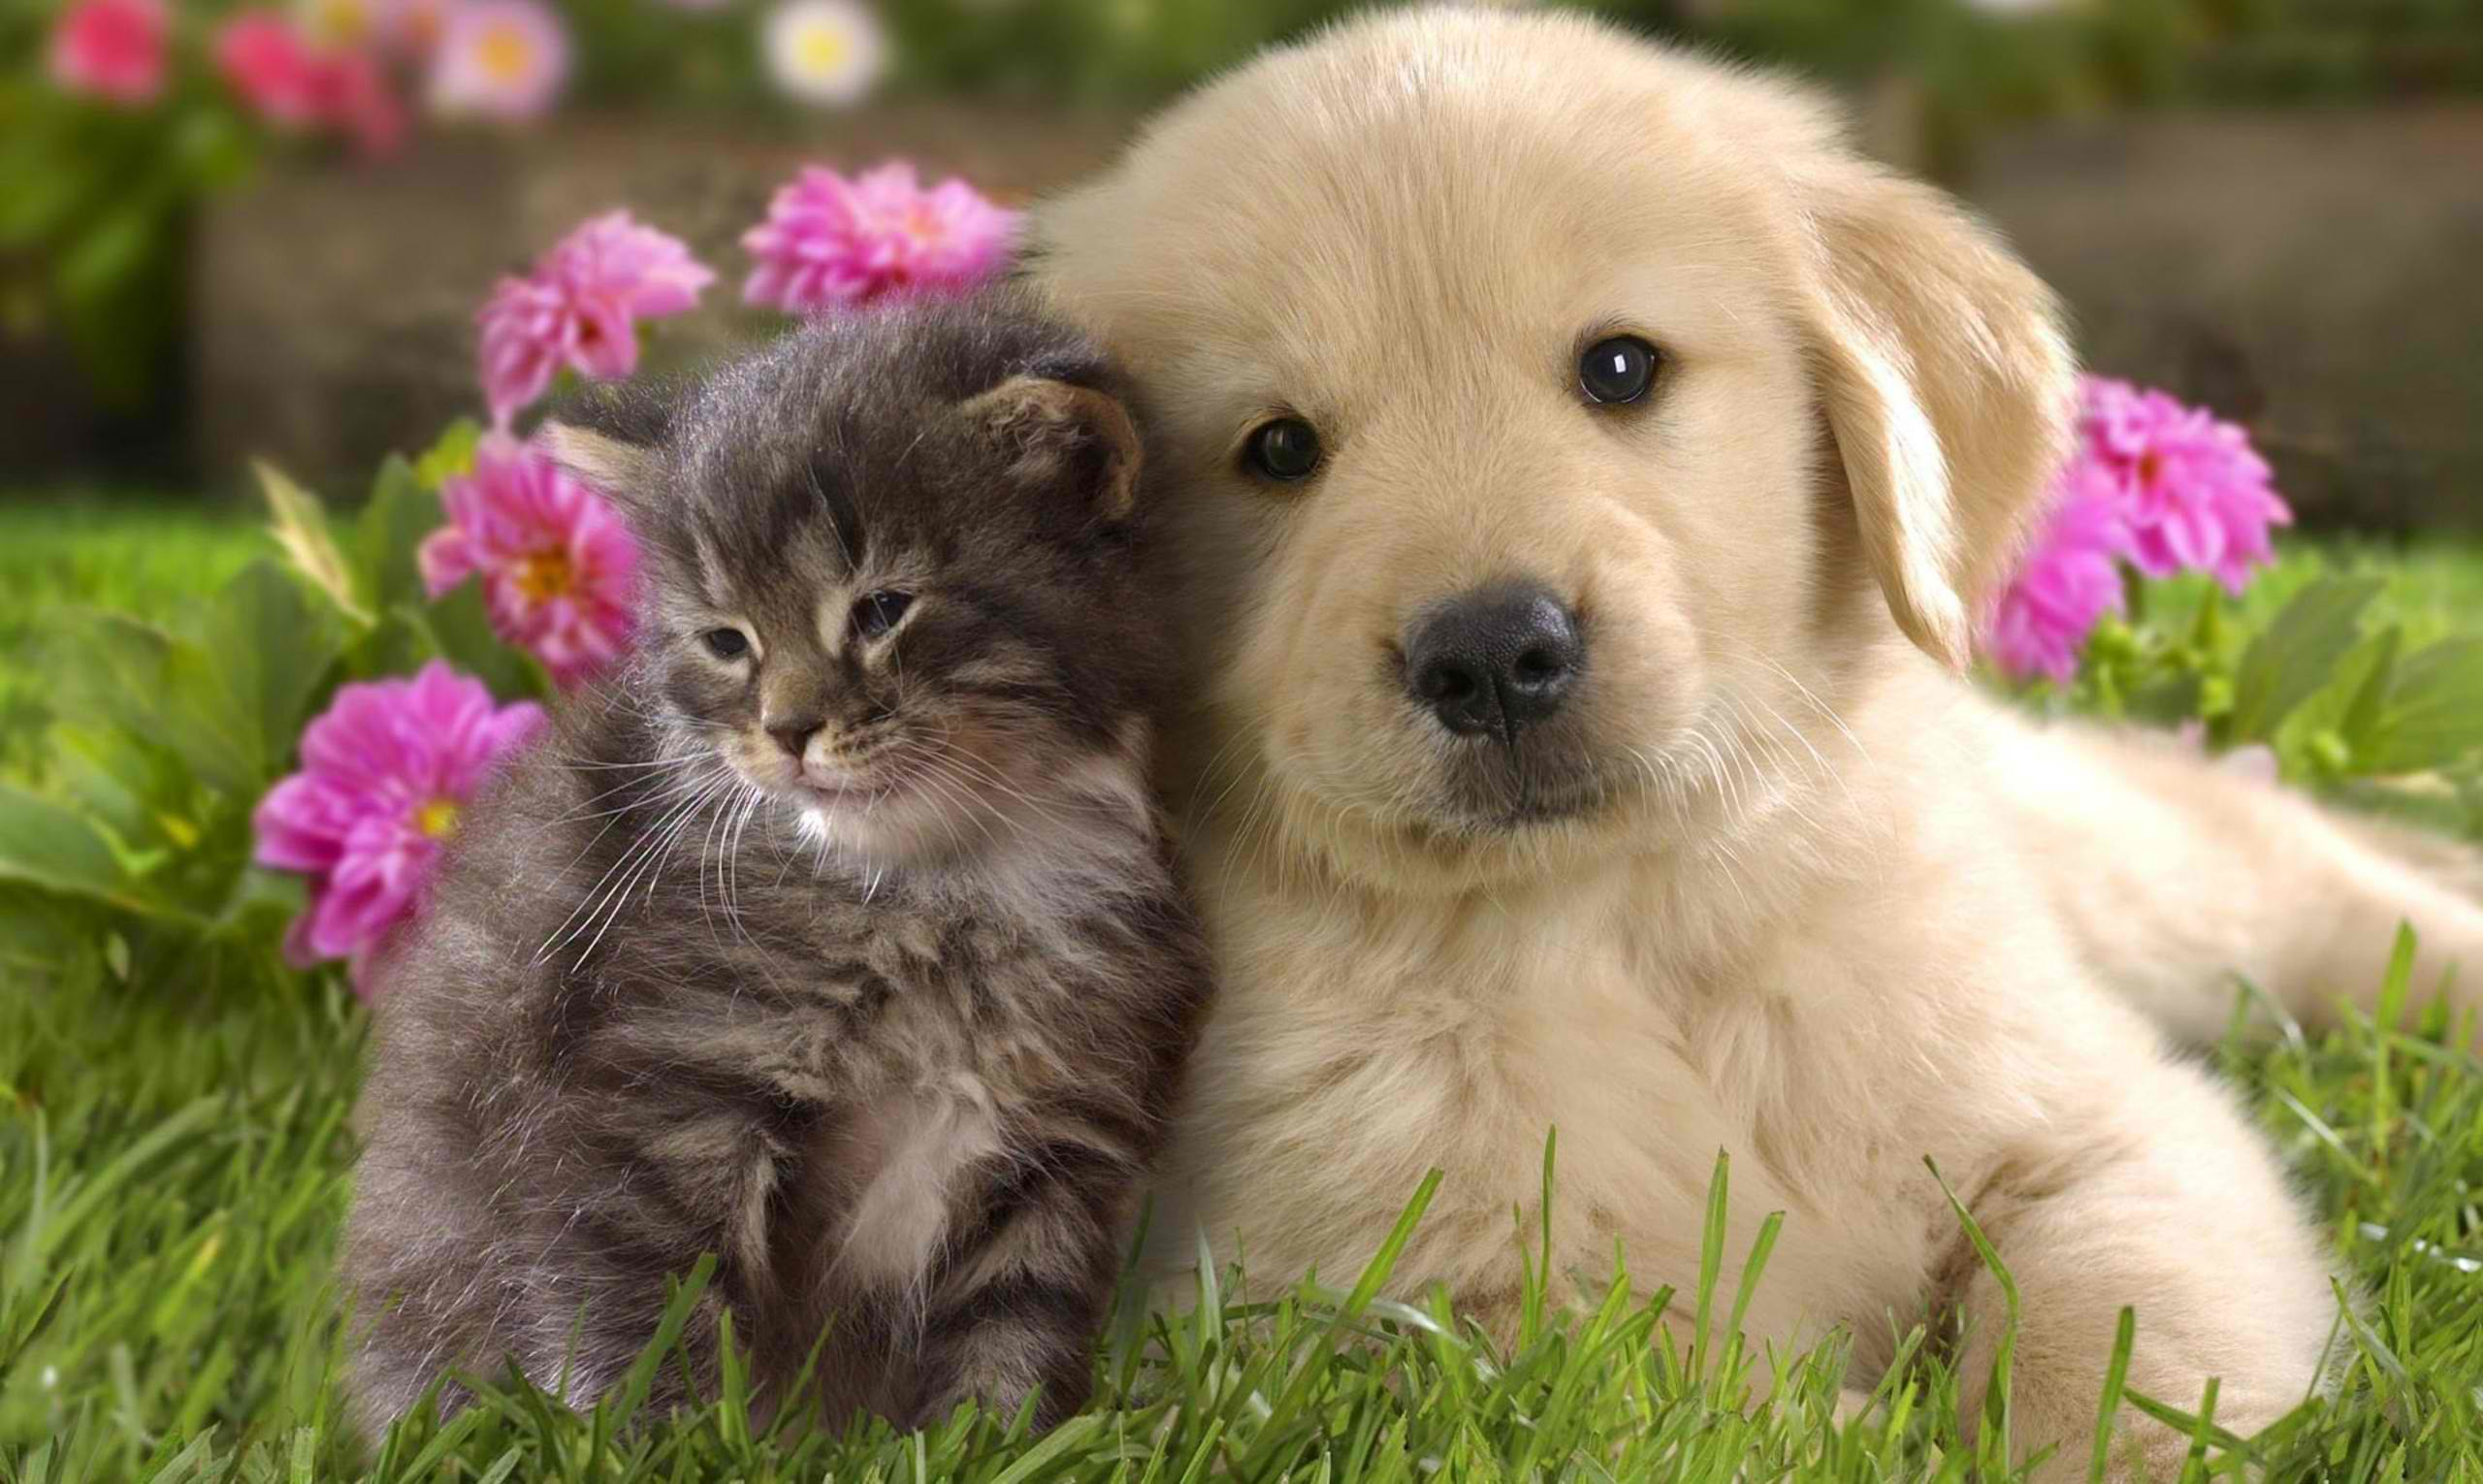
\includegraphics[height=7.5cm,width=10cm]{../pics/puppy.png}
    \label{fig:stack}
  \end{figure}
\end{frame}

\begin{frame}
  \frametitle{Probleme, Probleme, Probleme...}

  \begin{itemize}
  \item Ein GIT Repo funktioniert nicht bei Änderungen von Upstream Modulen
  \item Andere Abteilungen sollen ihre Module unabhänging Testen
  \item Unittests sagen noch nichts aus wie sich der Code am Live-System verhält
  \item Wir sollten eigentlich das Zusammenspiel aller Modele testen (Forge und eigene)
  \end{itemize}
\end{frame}

\begin{frame}
  \frametitle{Was haben wir geplant?}

  \begin{itemize}
  \item r10k für Deployment
  \item Ein Repository pro Module
  \item Puppet coverage tests
  \item Acceptance Tests mit Beaker
  \end{itemize}
\end{frame}


\end{document}